\chapter{Privacidade Não Morreu}
\label{les:19}

\begin{chapquote}{Lewis Carroll, \textit{Alice no País das Maravilhas}}
	Todos os jogadores jogaram juntos, sem esperar por turno, e discutiram 
	gritando a plenos pulmões, e em poucos minutos Rainha, em uma paixão 
	furiosa, batendo os pés e gritando \enquote{cortem a cabeça dele!} e 
	\enquote{cortem a cabeça dela!} mais ou menos a cada minuto.
\end{chapquote}

Se você acreditar nos especialistas, a privacidade morreu desde os anos 80
\footnote{\url{https://bit.ly/privacy-is-dead}}. A invenção do Bitcoin por um 
pseudônimo e outros eventos na história corrente mostram que isso não é verdade.
Privacidade está viva, mesmo que não seja fácil escapar de um Estado de vigilância. 

Satoshi fez um grande esforço para encobrir seus rastros e esconder
sua identidade. Dez anos depois, ainda não se sabe se Satoshi Nakamoto era uma pessoa 
solteira, um grupo de pessoas, homem, mulher ou uma IA que viaja no tempo que se 
autoinicializou a si mesmo para dominar o mundo. Teorias da conspiração à parte, Satoshi 
escolheu se identificar como um japonês, e é por isso que eu não suponho, mas respeito seu 
gênero escolhido e me refiro a ele como \textit{ele}. 

\begin{figure}
  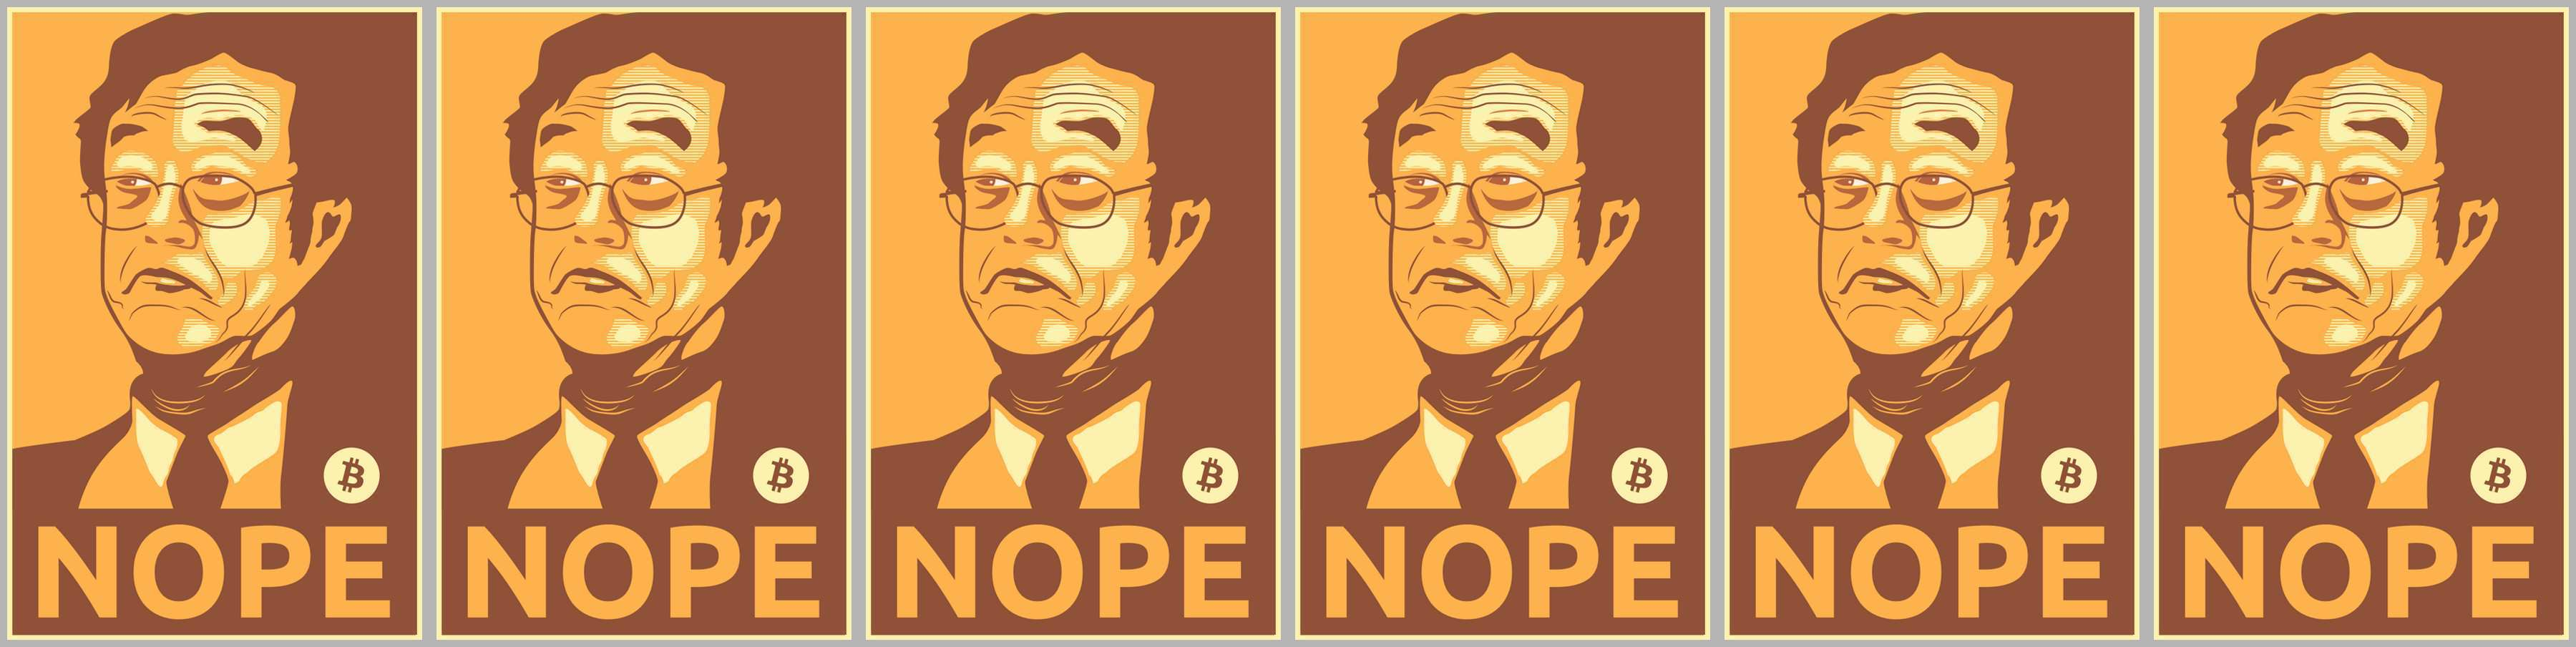
\includegraphics{assets/images/nope.png}
  \caption{Eu não sou Dorian Nakamoto.}
  \label{fig:nope}
\end{figure}

Qualquer que seja a sua identidade real, Satoshi teve sucesso em escondê-la. 
Ele deu um exemplo encorajador para todo mundo que deseja ficar anônimo: 
é possível ter privacidade online.

\begin{quotation}\begin{samepage}
\enquote{Encriptação Funciona. Um sistema de criptografia propriamente implementado é 
	uma das poucas coisas em que se pode confiar.}
\begin{flushright} -- Edward Snowden\footnote{Edward Snowden, respondendo à perguntas dos leitores \cite{snowden}}
\end{flushright}\end{samepage}\end{quotation}

Satoshi não foi o primeiro inventor anônimo ou pseudônimo, e ele não vai ser o último.
Alguns imitaram seu estilo de publicação pseudônima, como Tom Elvis Yedusor, criador da 
MimbleWimble~\cite{mimblewimble-origin} enquanto outros publicaram provas matemáticas avançadas 
e permaneceram completamente anônimos~\cite{4chan-math}.

Esse mundo em que vivemos é estranho. Um mundo onde identidade é opcional, 
contribuições são aceitas baseadas no mérito, e pessoas podem colaborar e transacionar livremente.
Vai demorar ainda algum tempo para me ajustar e ficar confortável com esses paradigmas, mas eu acredito 
fortemente que todas essas coisas tem potencial de mudar o mundo para melhor.

Nós sempre devemos lembrar que privacidade é um direito humano\footnote{Universal 
	Declaration of Human Rights, \textit{Article 12}.~\cite{article12}} fundamental. 
E enquanto as pessoas exercerem e defenderem 
esses direitos, a batalha por privacidade está longe de acabar.

\paragraph{Bitcoin me ensinou que a privacidade não morreu.}

% ---
%
% #### Down the Rabbit Hole
%
% - [Universal Declaration of Human Rights][fundamental human right] by the United Nations
% - [A lower bound on the length of the shortest superpattern][anonymous] by Anonymous 4chan Poster, Robin Houston, Jay Pantone, and Vince Vatter
%
% [since the 80ies]: https://books.google.com/ngrams/graph?content=privacy+is+dead&year_start=1970&year_end=2019&corpus=15&smoothing=3&share=&direct_url=t1%3B%2Cprivacy%20is%20dead%3B%2Cc0
% [time-traveling AI]: https://blockchain24-7.com/is-crypto-creator-a-time-travelling-ai/
% ["I am not Dorian Nakamoto."]: http://p2pfoundation.ning.com/forum/topics/bitcoin-open-source?commentId=2003008%3AComment%3A52186
% [MimbleWimble]: https://github.com/mimblewimble/docs/wiki/MimbleWimble-Origin
% [anonymous]: https://oeis.org/A180632/a180632.pdf
% [fundamental human right]: http://www.un.org/en/universal-declaration-human-rights/
%
% <!-- Wikipedia -->
% [alice]: https://en.wikipedia.org/wiki/Alice%27s_Adventures_in_Wonderland
% [carroll]: https://en.wikipedia.org/wiki/Lewis_Carroll
